\documentclass[danish]{article}
\usepackage[T1]{fontenc}
%\usepackage[utf8]{inputenc}

\usepackage[danish]{babel}
%\usepackage[danish]{isodate}
\usepackage[dvipsnames,table]{xcolor}

\usepackage{ulem}
%https://mirrors.dotsrc.org/ctan/macros/luatex/latex/emoji/emoji-doc.pdf
%\usepackage{emoji}
\usepackage{amsmath,amsfonts,amssymb,amsthm}
\usepackage{multirow}
\usepackage{lilyglyphs} %https://www.ctan.org/pkg/lilyglyphs
\usepackage{boldline}
\usepackage{etoolbox}
\usepackage{xstring}
\usepackage{csquotes}
%\usepackage{datetime}
\usepackage{microtype}
%\usepackage{newspaper}
\usepackage{yfonts}  % used for the paper title font
\usepackage{fontspec}
%\usepackage{
%\date{\today}

%\SetPaperName{Solsikke Tidende}
%\SetPaperLocation{Santiago de Cali}
%\SetPaperSlogan{\clefG \hspace{0.15cm} \textbf{$Cipher_{Caesar}(_3)$} \hspace{0.15cm} \clefG}
%\SetPaperPrice{}

\DeclareFontFamily{LYG}{bigygoth}{}
\DeclareFontShape{LYG}{bigygoth}{m}{n}{<->s*[2.5]ygoth}{}

\setlength\topmargin{-48pt} 		% article default = -58pt
\setlength\headheight{0pt}  		% article default = 12pt
\setlength\headsep{34pt}		% article default = 25pt
\setlength\marginparwidth{-20pt}	% article default = 121pt
\setlength\textwidth{7.0in}		% article default = 418pt
\setlength\textheight{9.5in}		% article default = 296pt
\setlength\oddsidemargin{-30pt}



\def\papername{Solsikke Tidende}
\def\headername{Solsikke Tidende}   % because of the yfonts you may need both papername and headername
\def\paperlocation{København}
\def\musagsduhint{{\footnotesize \clefG} \hspace{0.15cm} \textbf{$Cipher_{Caesar}(4)$} \hspace{0.15cm} {\footnotesize \clefG}}
\newcommand\muzait{{\scriptsize\twoBeamedQuavers}\,}

\newcommand\muzaselection[3]{
  \paragraph{}
  {\fontfamily{lmr}\selectfont
  \textit{
    \muzait 
    {\Large\textbf{\StrLeft{#1}{1}}}\StrGobbleLeft{#1}{1}\, 
     \muzait} (#2) \\
  {\scriptsize
   \textit{
      \blockquote{#3}
    }
  }
}}

\def\paperprice{0 DKK}

\newcounter{volumeno}
\setcounter{volumeno}{66}
\newcounter{issueno}
\setcounter{issueno}{27}



\usepackage{times}
\usepackage{graphicx}
\usepackage{multicol}
\usepackage{picinpar}

\usepackage{lipsum}


%\colorlet{cfernando}{LightSteeleBlue3}
\definecolor{cfernando}{RGB}{38,40,74}
\definecolor{canna}{RGB}{164, 39, 168}
\definecolor{csune}{RGB}{125,21,21}
\definecolor{cmaria}{RGB}{245, 66, 120}

\definecolor{cother}{RGB}{103, 103, 152}


\newcommand\sayanna[1]{
  {\fontfamily{lmr}\selectfont \color{canna}{\textit{- #1}}}
}

\newcommand\saymaria[1]{
  {\large
     {\setmainfont{Gabriola} \color{cmaria}{\textit{- #1}}}
  }
}


\newcommand\sayfernando[1]{
  {\fontfamily{lmr}\selectfont \color{cfernando}{\textit{- #1}}}
}

\newcommand\saysune[1]{
  {\setmainfont{Ink Free} \color{csune}{\textit{- #1}}}
}

\newcommand\sayother[1]{
  {\fontfamily{lmr}\selectfont \color{cother}{\textit{- #1}}}
}



\newcommand\translatedfrom[1]{
 \begin{center}
  {\fontfamily{lmdh}\selectfont
  {\textit{oversat fra #1}}
  }
 \end{center}

}


\renewcommand{\maketitle}{
  \thispagestyle{empty}
  \vspace*{-40pt}
  \begin{center}
  \hfill
  {\textgoth
   {\huge 
     \usefont{LYG}{bigygoth}{m}{n} \papername
   }
  }\hfill%	
  \raisebox{12pt}{
   \textbf{
    \footnotesize 
    \paperlocation
   }
  }\\
  \vspace*{0.1in}
  \rule[0pt]{\textwidth}{0.5pt}\\
  {\small 
    VOL.\MakeUppercase{\roman{volumeno}}
    \ldots No. \arabic{issueno}
   } \hfill 
   \MakeUppercase{\small  19. december 2023} 
   \hfill {\small }\\
  \rule[6pt]{\textwidth}{1.2pt}
  \end{center}
  \pagestyle{plain}
}

\def\ps@plain{%
  \renewcommand\@oddfoot{}%					% empty recto footer
  \let\@evenfoot\@oddfoot						% empty verso footer
  \renewcommand\@evenhead
  {\parbox{\textwidth}{\vspace*{4pt}
  {\small VOL.\MakeUppercase{\roman{volumeno}}\ldots No.\arabic{issueno}}\hfill\normalfont\textbf{\headername}\quad\MakeUppercase{\textit\today}\hfill\textrm{\thepage}\\
  \rule{\textwidth}{0.5pt}
  \vspace*{12pt}}}%
  \let\@oddhead\@evenhead
}
		

\newcommand\headline[1]{
  {\fontfamily{lmdh}\selectfont
    \begin{center} #1\\ %
    \rule[3pt]{0.4\hsize}{0.5pt}\\ \end{center} \par
  }
}

\newcommand\byline[2]{
  {\fontfamily{lmdh}\selectfont
  \begin{center} #1 \\%
  {\footnotesize\bf af \MakeUppercase{#2}} \\ %
  \rule[3pt]{0.4\hsize}{0.5pt}\\ \end{center} \par
  }
}


\newcommand\closearticle{{\begin{center}\rule[6pt]{\hsize}{1pt}\vspace*{-16pt}
			\rule{\hsize}{0.5pt}\end{center}}}



\begin{document}


\maketitle
\fontfamily{phv}\selectfont

\begin{multicols}{2}
\byline{Back in the game}{Fernándo Sanchez}
\subsection*{Kærligheden}

Hvis min tro på menneskeheden var tanken på en bil, kørte den på dampene da jeg væltede ned af CMO’ens opgang, og efterfølgende blev forfulgt i godt 2 kilometer igennem den københavnske forstad af en kun-fornødent påklædt galning, der skiftevis råbte mig an med de mest nederdrægtige gloser, skiftevis undskyldte og råbte “BUM”, skiftevis faldt om på jorden i voldsomme krampeanfald.\\

Det siges at man først finder friheden når man har mistet alt. Den aften mistede jeg noget af det sidste jeg havde tilbage: “håbet” og fandt som ved en håndsrækning fra Gud noget der var endnu bedre end friheden: \textbf{KÆRLIGHEDEN}.  Jeg mødte Maria i toget på vej tilbage mod København, da en livstræt tog-kontrollør var i færd med at udskrive mig en bøde.\\

\saymaria{Der var du Henrik! Jeg har ledt alle steder efter dig… du ved godt at du ikke bare sådan må gå fra mig uden at sige hvor du går hen!\\
Nej, hør nu her, er du ved at give denne mand en bøde… kan du da ikke se at han er socialt handikappet?}
\saymaria{\textit{(Henvendt til mig)} du burde altså huske Solsikkesnoren når du går ud!}\\

Som en Guds engel der kærligt uddeler Herrens beskyttende nåde, lagde hun nu forsigtigt en Solsikkesnor om halsen på mig. Togkontrolløren syntes en smule ubekvem ved situationen, og jeg kunne mærke en vægtskål skifte til vores favør. Jeg vidste ikke helt hvad Solsikkesnoren betød, men inspireret af mit seneste møde med CMO’en, vred jeg nu min krop i pludselige spasmer.\\

\saymaria{Kom Henrik, vi skal af her, og så slipper vi for den VÆMMELIGE mand og hans VÆMMELIGE bøder} sagde Maria idet hun flåede mig op fra sæddet og med ud på Vanløse St. \\
\saymaria{Hold kæft en idiot} råbte hun idet toget kørte forbi os.\\
\sayfernando{\textbf{BUM}} istemte jeg muntert.\\

Dagene siden torsdag, har jeg tilbragt på en lyserød sky (eller en lejlighed i Vanløse) i selskab med den dejligste kvinde i verden, piller i alle mulige farver og begyndende hudløshed.\\


Det var først søndag morgen at jeg tog mig sammen til at tænde min telefon igen, for nødtvungent at forholde mig til omverdenen - og især OOCMO - igen (figur \ref{fig:convos})




\subsection*{Alperne}

Jeg stod foran føtex kl. 17:56, og som punktligheden selv kom Anna på slaget 18:00.\\
\sayanna{Den her slutrunde har overgået alle vores forventninger! Konkurrencen med især OOCMO@Danske Bank har tvunget os til at gå spritnye veje denne jul, og resultatet er ikke til at tage fejl af: vi vidste at vi havde en vinder med Musical Contest; det er et efterhånden velkendt format for os, og vores brugere har denne gang mestendels stemt rationelt, men opbakningen til Team Contest har været FORMIDABEL! Vi har ramt et format som har lokket de mest drevne - men samtidigt også mest korrumperede - sider af den menneskelige natur frem. Vi har set folk der har snydt i Find Nissen, og tilmed været nødt til at diskvalificere et hold på et tidspunkt!}


\sayfernando{Det må jeg give jer, det lyder som noget af en succes!}


\sayanna{Kæmpe! Men vi er kun lige kommet til Alperne, og set vores første kategori 1 bjerg. I morgen (tirsdag) har vi et kategori 2 bjerg, og onsdag forventer vi at finde vinderen af Team Contest når vi går \hspace{5px} \textbf{Hors catégorie}. Vi har set en kraftpræstation fra nogle meget dedikerede indvidualister som alle ligger meget lunt til at vinde den gule trøje, men det er vigtigt for mig at påpege, at såvel Team Contest som den indviduelle konkurrence er \textbf{PIV-åbne}, for dem der stadigvæk har saft i benene!}\\

\sayfernando{Hold da op! Er alle holdene stadigvæk med i løbet om førstepladsen?}\\
\sayanna{Nej! Vi har indset at der er meget stor forskel på modenheden af de deltagende teams, og vi må desværre sande at nogle teams bare ikke har niveauet til at deltage på det her plan. Til næste slutrunde-arrangement under OOCMO, kommer vi til at stille større krav til de deltagende hold, og vi kommer til at frasortere de teams og deltagere som ikke har performet…}\\

Jeg mærkede pludselig noget spidst stikke mig i siden
\saysune{\textbf{Hænderne op, det er politiet! Jesper ... mmmm... Jespersen, du er anholdt for æresløst at stikke af fra en kamp til døden, i værste fald strafbart ved Blodørnen}} erklærede en dyb stemne højt. Selv uden de åbenlyse ledetråde, havde bunden af vanvid i mandens stemme ikke efterladt mig med nogen tvivl om dens ejermand. De forbipasserende vendte sig for at se hvad der skete.\\

\saysune{\textbf{Hvil I blot trygt kære Pøbel! Ordensmagten har styr på sagerne, og vil nu kropsvisitere truslen og sikre at den ikke har sprængstoffer eller andre skadelige sager på sig!}}\\

Jeg vidste jo nok hvad han var ude efter, så jeg sparede ham besværet og rakte ham glasset med stryknin.

\saysune{\textbf{Der ser i Befolkning! Det Gode vinder endnu engang… for det har Bamse selv bestemt!}}\\

Da jeg vendte mig for at kigge efter ham, kunne jeg se CMO’en gadedrengeløbe sig muntert igennem de travle julemasser, med pilleglasset triumferende rejst i vejret.


\byline{Reportage fra en krigszone}{Thorkild Tjärnsten}
Havde jeg for 2 måneder siden bedt dig, kære læser, om at male mig et billede af Vesterbro en uge inden Juleaften, er jeg sikker på at det billede havde indeholdt letpåklædte skønheder fra alle verdenshjørner, glade gadesælgere og fornøjede forretningsfolk på vej hjem til kernefamilien efter en hård dag på arbejdet og en velfortjent optankning på overskuds-kontoen fra førnævnte. Billedet havde næppe indeholdt finansfolk på motorcykler, julemænd med flækøkser, gader indsmurt i blod og udtrådte avocadoer, og skræmte beboere der kigger magtesløse til bag køkkenvinduerne imens politiet ingen steder er at finde, men det er nu engang den virkelighed vi har levet i de sidste par uger.\\
Vi lavede en hurtig voxpop med én af de få lovlydige mennesker vi mødte på Istedgade.

\sayother{(\textbf{Artur Jävnström - studerende} ) Den her situation er så mega uholdbar! Jeg kom til København for at studere, møde nye mennesker og bede kvinder på Snapchat om at sende mig billeder af deres bryster; hvis jeg ville have blodsindsmurte voldsjulemænd og skræmte prostituerede var jeg jo blevet i Randers! Mine venner og jeg fra studiet holdte julefrokost i weekenden, og det var umuligt at støve blæs af både den ene og anden art op. Uhørt! Og hvor er politiet? Er det for pokker ikke os de bliver betalt for at beskytte? Vi er cremen af Danmarks ungdom! Det er os der kommer til at finansiere det her velfærdsgilde lige om lidt! Min fætter der er færdselsbetjent i Holbæk siger at alle senior-officerer i den københavnske politi-styrke er taget til Lanzarote på ubestemt tid!?!}


\byline{Blod-mysteriet}{Susan Saxing}
Natten til mandag blev endnu en ung mand der på ulyksagelig vis havde mistet alt sit blod, fundet død foran Emdrupparkens Idrætsanlæg. Derved er dødstallet oppe på 7 siden de makabre fund begyndte for ca. 3 uger siden. Solsikke Tidendes udsendte tog en snak med junior kriminalbetjent Noah Golt Spalt-Schläger.\\

\sayother{Jeg vil godt have at du opgører mig som \textbf{Kriminalkommissær Golt Spalt-Schläger}. Vil du gøre det? Jeg er nemlig sikker på at ``dem med stjerner på skuldrene'' nok skal belønne mig med en lille forfremmelse når jeg har knækket den her sag lige om lidt. Ser du... jeg har ``Scherlocket''... Jeg spurgte migselv: ``hvad ville Scherlock gøre?'', og så gik jeg ud og snakkede med beboerne i området, og det har så sandelig båret pote. Jeg har fra meget pålidelig kilde, at der kort tid før de gamle mænd begyndte at tabe blodet, er blevet rejst \textbf{5G antenner} i området. Coincidence? ``I think not my dear Watson!''}


\end{multicols}{2}

\begin{figure}
	\centering
		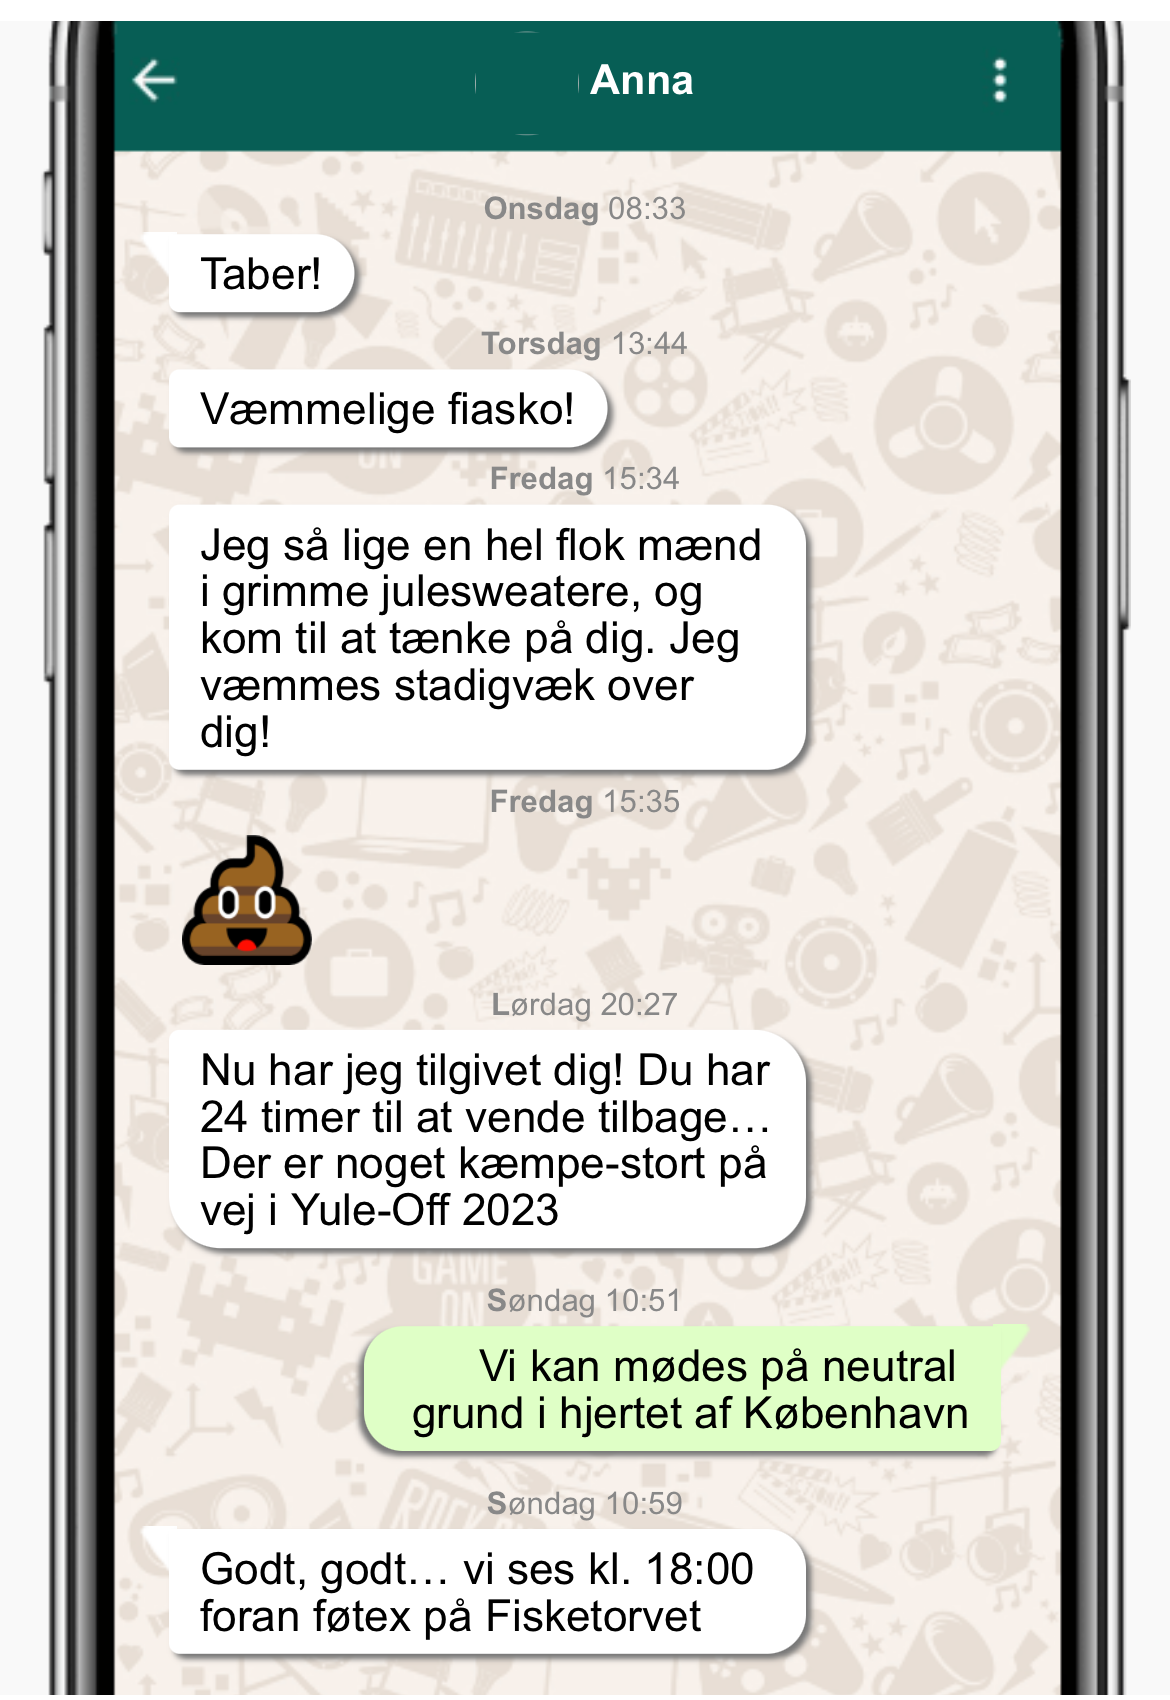
\includegraphics[width=0.25\linewidth]{convo-anna.png}
		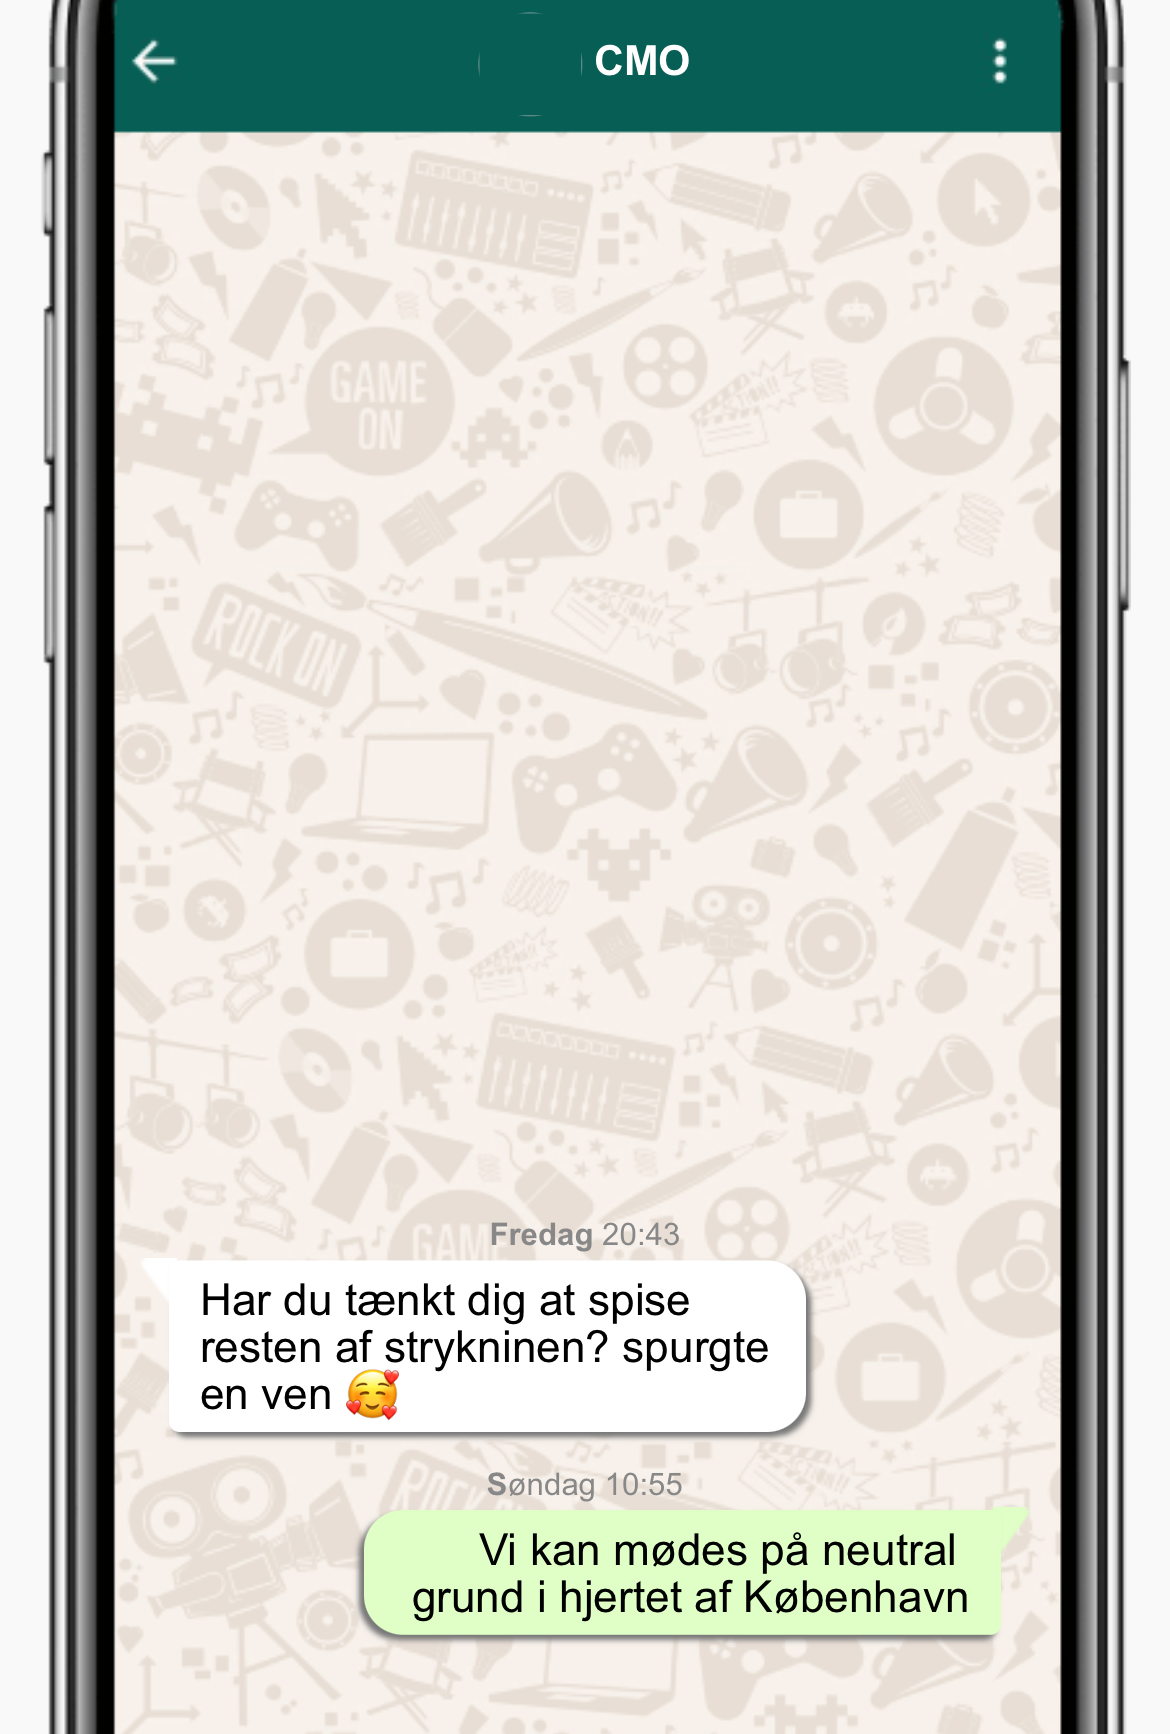
\includegraphics[width=0.25\linewidth]{convo-sune.png}
		
	\caption{Besked-tråde med OOCMO}
	\label{fig:convos}
\end{figure}



\end{document}